% Options for packages loaded elsewhere
\PassOptionsToPackage{unicode}{hyperref}
\PassOptionsToPackage{hyphens}{url}
%
\documentclass[
]{article}
\usepackage{lmodern}
\usepackage{amssymb,amsmath}
\usepackage{ifxetex,ifluatex}
\ifnum 0\ifxetex 1\fi\ifluatex 1\fi=0 % if pdftex
  \usepackage[T1]{fontenc}
  \usepackage[utf8]{inputenc}
  \usepackage{textcomp} % provide euro and other symbols
\else % if luatex or xetex
  \usepackage{unicode-math}
  \defaultfontfeatures{Scale=MatchLowercase}
  \defaultfontfeatures[\rmfamily]{Ligatures=TeX,Scale=1}
\fi
% Use upquote if available, for straight quotes in verbatim environments
\IfFileExists{upquote.sty}{\usepackage{upquote}}{}
\IfFileExists{microtype.sty}{% use microtype if available
  \usepackage[]{microtype}
  \UseMicrotypeSet[protrusion]{basicmath} % disable protrusion for tt fonts
}{}
\makeatletter
\@ifundefined{KOMAClassName}{% if non-KOMA class
  \IfFileExists{parskip.sty}{%
    \usepackage{parskip}
  }{% else
    \setlength{\parindent}{0pt}
    \setlength{\parskip}{6pt plus 2pt minus 1pt}}
}{% if KOMA class
  \KOMAoptions{parskip=half}}
\makeatother
\usepackage{xcolor}
\IfFileExists{xurl.sty}{\usepackage{xurl}}{} % add URL line breaks if available
\IfFileExists{bookmark.sty}{\usepackage{bookmark}}{\usepackage{hyperref}}
\hypersetup{
  pdftitle={Medical Expenses},
  pdfauthor={Nima Jamshidi \& Diana Lin},
  hidelinks,
  pdfcreator={LaTeX via pandoc}}
\urlstyle{same} % disable monospaced font for URLs
\usepackage[margin=1in]{geometry}
\usepackage{longtable,booktabs}
% Correct order of tables after \paragraph or \subparagraph
\usepackage{etoolbox}
\makeatletter
\patchcmd\longtable{\par}{\if@noskipsec\mbox{}\fi\par}{}{}
\makeatother
% Allow footnotes in longtable head/foot
\IfFileExists{footnotehyper.sty}{\usepackage{footnotehyper}}{\usepackage{footnote}}
\makesavenoteenv{longtable}
\usepackage{graphicx,grffile}
\makeatletter
\def\maxwidth{\ifdim\Gin@nat@width>\linewidth\linewidth\else\Gin@nat@width\fi}
\def\maxheight{\ifdim\Gin@nat@height>\textheight\textheight\else\Gin@nat@height\fi}
\makeatother
% Scale images if necessary, so that they will not overflow the page
% margins by default, and it is still possible to overwrite the defaults
% using explicit options in \includegraphics[width, height, ...]{}
\setkeys{Gin}{width=\maxwidth,height=\maxheight,keepaspectratio}
% Set default figure placement to htbp
\makeatletter
\def\fps@figure{htbp}
\makeatother
\setlength{\emergencystretch}{3em} % prevent overfull lines
\providecommand{\tightlist}{%
  \setlength{\itemsep}{0pt}\setlength{\parskip}{0pt}}
\setcounter{secnumdepth}{-\maxdimen} % remove section numbering

\title{Medical Expenses}
\author{Nima Jamshidi \& Diana Lin}
\date{3/6/2020}

\begin{document}
\maketitle

{
\setcounter{tocdepth}{2}
\tableofcontents
}
\hypertarget{introduction}{%
\subsection{Introduction}\label{introduction}}

The dataset we have chosen to work with is the ``Medical Expenses''
dataset used in the book
\href{https://www.amazon.com/Machine-Learning-R-Brett-Lantz/dp/1782162143}{Machine
Learning with R}, by Brett Lantz. This dataset was extracted from
\href{https://www.kaggle.com/mirichoi0218/insurance/home}{Kaggle} by
Github user
\href{https://gist.github.com/meperezcuello}{@meperezcuello}. The
information about this dataset has been extracted from their
\href{https://gist.github.com/meperezcuello/82a9f1c1c473d6585e750ad2e3c05a41}{GitHub
Gist}.

This dataset is very interesting as the USA does not have universal
healthcare, and is known for bankrupting its citizens with hospital
visits despite having insurance. It will be interesting to see the
relationship between characteristics of a beneficiary, such as
\texttt{BMI} and \texttt{Smoking} status, and the \texttt{charges}
incurred.

\hypertarget{research-question}{%
\subsection{Research Question}\label{research-question}}

In this study, we are analyzing the data to find a relationship between
the features and the amount of insurance cost.

Does having an increased BMI increase your insurance costs? What about
age? Number of dependents? Smoking status? Are certain areas of the USA
associated with higher insurance costs?

In order to answer the questions above we're planning to perform a
linear regression analysis and plot the regression line and relevant
variables. The variables need to be normalized before performing the
regression analysis.

\hypertarget{data-description}{%
\subsection{Data Description}\label{data-description}}

This dataset explains the medical insurance costs of a small sample of
the USA population. Each row corresponds to a beneficiary. Various
metadata was recorded as well.

The columns (except the last one) in this dataset correspond to
metadata, where the last column is the monetary charges of medical
insurance. Here are the possible values for each of the columns:

\begin{longtable}[]{@{}lll@{}}
\toprule
\begin{minipage}[b]{0.27\columnwidth}\raggedright
Variable\strut
\end{minipage} & \begin{minipage}[b]{0.18\columnwidth}\raggedright
Type\strut
\end{minipage} & \begin{minipage}[b]{0.46\columnwidth}\raggedright
Description\strut
\end{minipage}\tabularnewline
\midrule
\endhead
\begin{minipage}[t]{0.27\columnwidth}\raggedright
Age\strut
\end{minipage} & \begin{minipage}[t]{0.18\columnwidth}\raggedright
integer\strut
\end{minipage} & \begin{minipage}[t]{0.46\columnwidth}\raggedright
the primary beneficiary's age in years\strut
\end{minipage}\tabularnewline
\begin{minipage}[t]{0.27\columnwidth}\raggedright
Sex\strut
\end{minipage} & \begin{minipage}[t]{0.18\columnwidth}\raggedright
factor\strut
\end{minipage} & \begin{minipage}[t]{0.46\columnwidth}\raggedright
the beneficiary's sex: \texttt{female} or \texttt{male}\strut
\end{minipage}\tabularnewline
\begin{minipage}[t]{0.27\columnwidth}\raggedright
BMI\strut
\end{minipage} & \begin{minipage}[t]{0.18\columnwidth}\raggedright
double\strut
\end{minipage} & \begin{minipage}[t]{0.46\columnwidth}\raggedright
the beneficiary's Body Mass Index, a measure of their body fat based on
height and weight (measured in kg/m2), an ideal range of 18.5 to
24.9\strut
\end{minipage}\tabularnewline
\begin{minipage}[t]{0.27\columnwidth}\raggedright
Children\strut
\end{minipage} & \begin{minipage}[t]{0.18\columnwidth}\raggedright
integer\strut
\end{minipage} & \begin{minipage}[t]{0.46\columnwidth}\raggedright
the number of dependents on the primary beneficiary's insurance
policy\strut
\end{minipage}\tabularnewline
\begin{minipage}[t]{0.27\columnwidth}\raggedright
Smoker\strut
\end{minipage} & \begin{minipage}[t]{0.18\columnwidth}\raggedright
factor\strut
\end{minipage} & \begin{minipage}[t]{0.46\columnwidth}\raggedright
whether or not the beneficiary is a smoker: \texttt{yes} or
\texttt{no}\strut
\end{minipage}\tabularnewline
\begin{minipage}[t]{0.27\columnwidth}\raggedright
Region\strut
\end{minipage} & \begin{minipage}[t]{0.18\columnwidth}\raggedright
factor\strut
\end{minipage} & \begin{minipage}[t]{0.46\columnwidth}\raggedright
the beneficiary's residential area in the USA: \texttt{southwest},
\texttt{southeast}, \texttt{northwest}, or \texttt{northeast}\strut
\end{minipage}\tabularnewline
\begin{minipage}[t]{0.27\columnwidth}\raggedright
Charges\strut
\end{minipage} & \begin{minipage}[t]{0.18\columnwidth}\raggedright
double\strut
\end{minipage} & \begin{minipage}[t]{0.46\columnwidth}\raggedright
the monetary charges the beneficiary was billed by health
insurance\strut
\end{minipage}\tabularnewline
\bottomrule
\end{longtable}

\hypertarget{exploring-the-dataset}{%
\subsection{Exploring the Dataset}\label{exploring-the-dataset}}

Here is a summary of the dataset, and the values of each variable:

\begin{longtable}[]{@{}lcccclcc@{}}
\toprule
& age & sex & bmi & children & smoker & region & charges\tabularnewline
\midrule
\endhead
& Min. :18.00 & female:662 & Min. :15.96 & Min. :0.000 & yes: 274 &
southwest:325 & Min. : 1122\tabularnewline
& 1st Qu.:27.00 & male :676 & 1st Qu.:26.30 & 1st Qu.:0.000 & no :1064 &
southeast:364 & 1st Qu.: 4740\tabularnewline
& Median :39.00 & & Median :30.40 & Median :1.000 & & northwest:325 &
Median : 9382\tabularnewline
& Mean :39.21 & & Mean :30.66 & Mean :1.095 & & northeast:324 & Mean
:13270\tabularnewline
& 3rd Qu.:51.00 & & 3rd Qu.:34.69 & 3rd Qu.:2.000 & & & 3rd
Qu.:16640\tabularnewline
& Max. :64.00 & & Max. :53.13 & Max. :5.000 & & & Max.
:63770\tabularnewline
\bottomrule
\end{longtable}

Next, we want to inspect the data set to see if there is any correlation
between the variables. From now on we want to consider charges as our
dependent variable. In order to analyze correlation between variables,
the ones that are categorical with two categories, are translated into
binery vectors. The only categorical variable with more than two
categories, is region. We split this variable into four different binery
vectors, each indicating if the sample data has category (1) or not (0).
After using dummy variables for sex, smoker, and region, according to
the correlogram below, smoker and charges has the strongest correlation
of 0.79. No high collinearity between independent variables is observed.

\begin{figure}
\centering
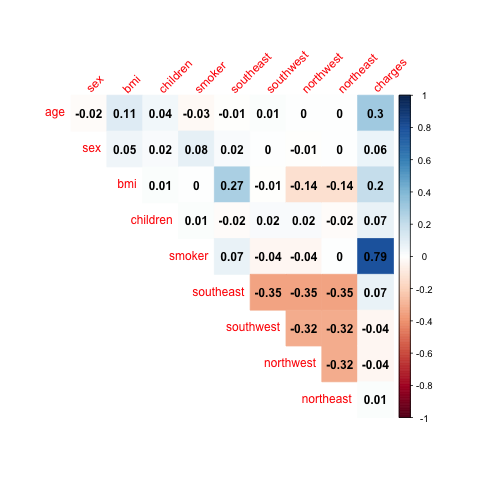
\includegraphics{../images/corrplot.png}
\caption{Correlogram}
\end{figure}

In order to to check if there is any cluster of data points, we use
faceted plot. While the data between regions and sex does not appear to
vary much, the smokers vs nonsmokers of each facet appear to cluster
together, with the non-smokers having an overall lower medical cost.

\begin{figure}
\centering
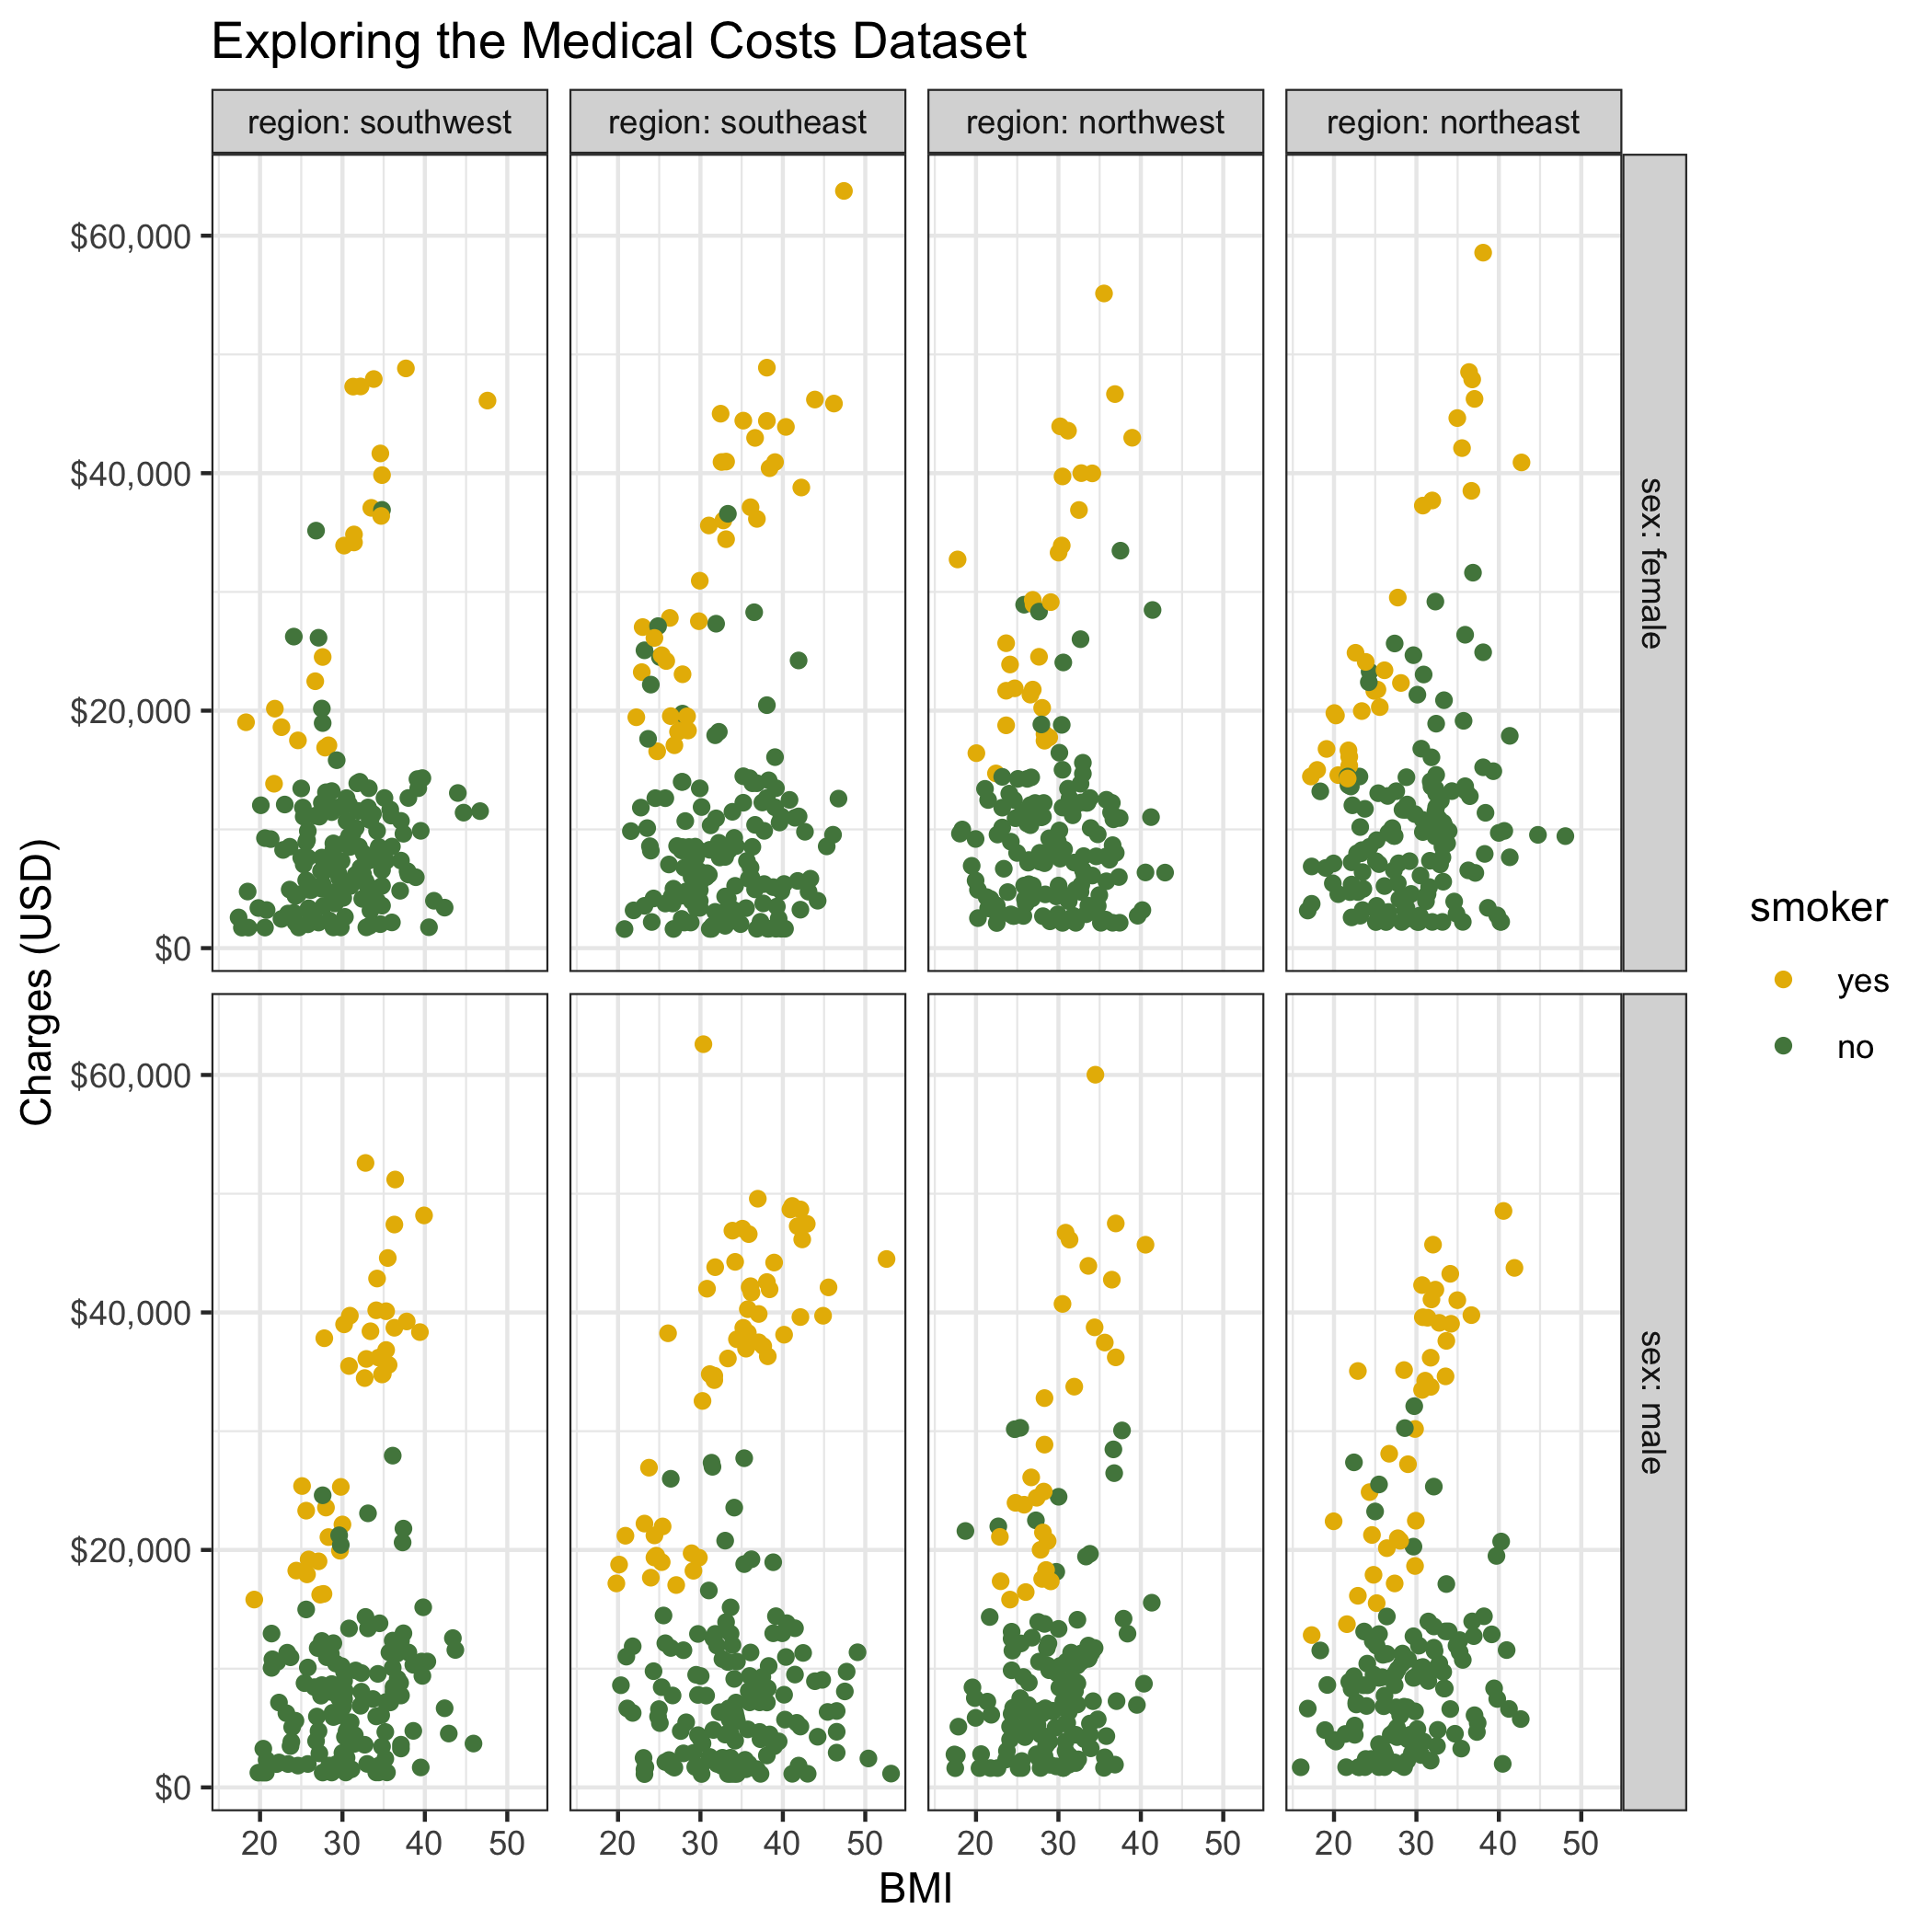
\includegraphics{../images/facet.png}
\caption{Facetted plot}
\end{figure}

How is the distribution of sex among different age groups? Looking at
the dataset, there appears to be more beneficiaries in the 20-60 age
range. The biggest difference in the number of beneficiaries from
different sex is seen in the 20-30 bracket.

\begin{figure}
\centering
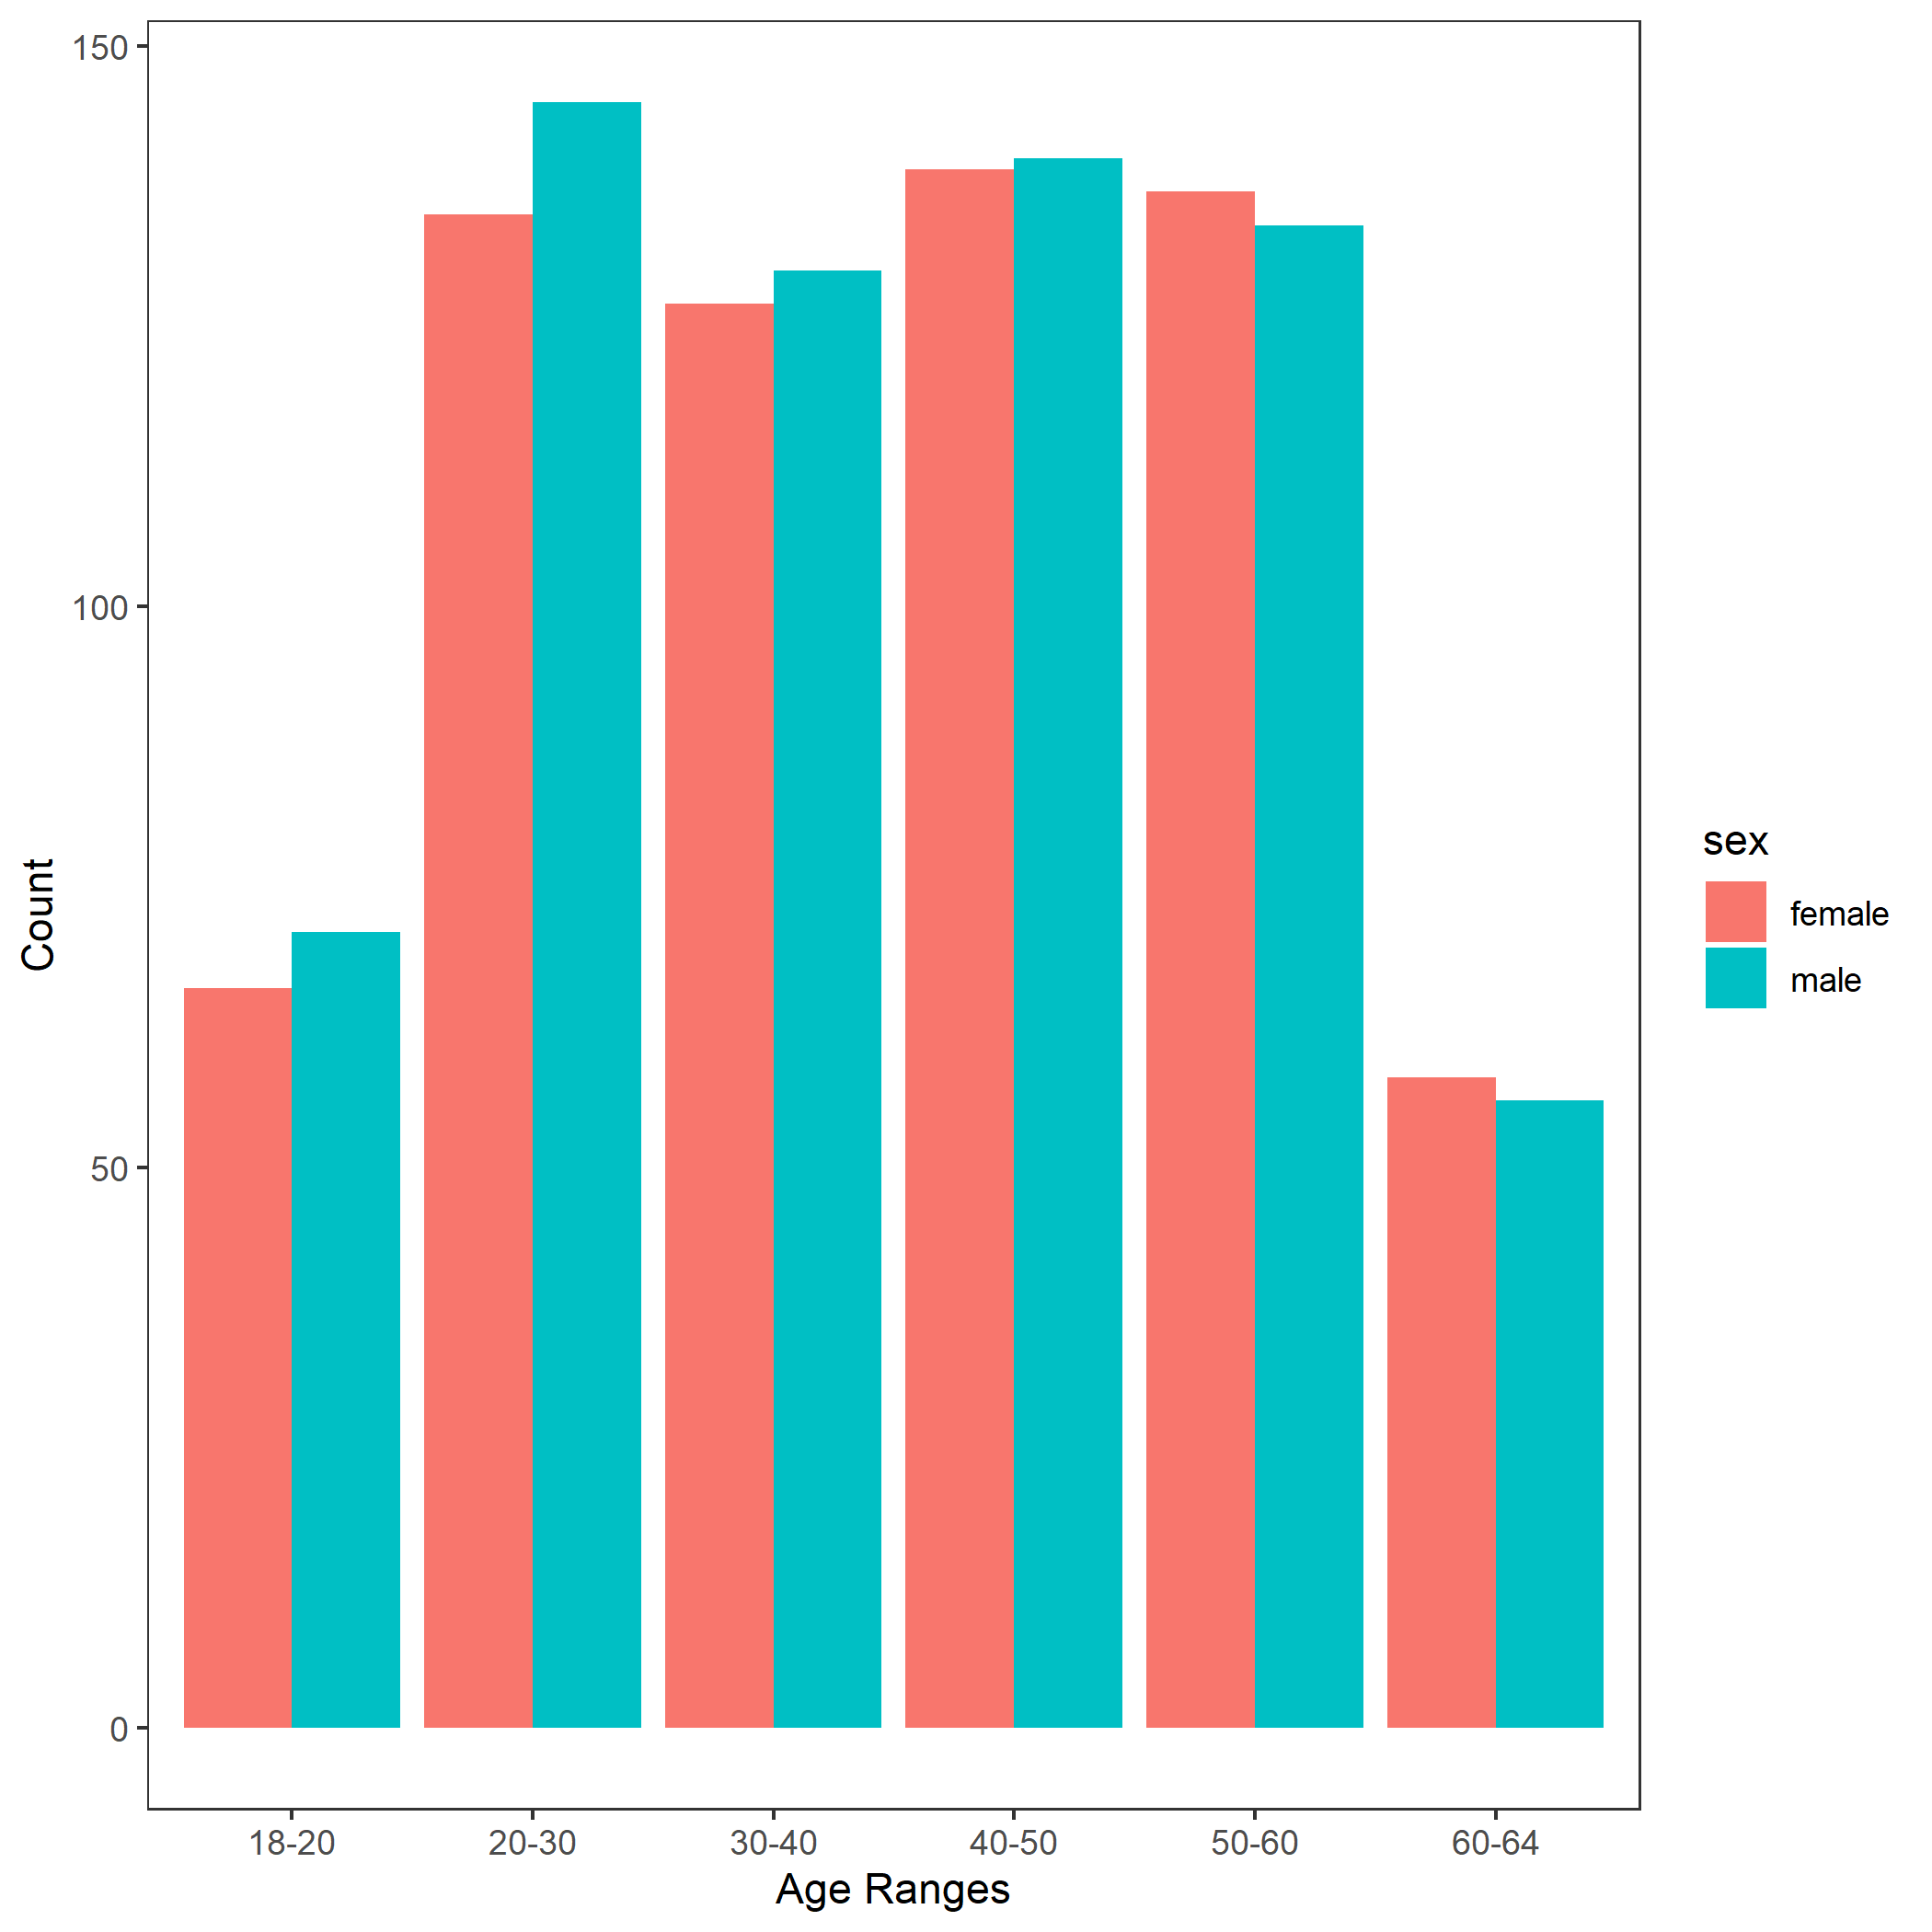
\includegraphics{../images/age_histogram.png}
\caption{Age histogram}
\end{figure}

How about the distribution of sex among the regions? This plot shows the
distribution of sex in each of the four regions. At a glance, the
dataset looks very even when it comes to sex, but there are slightly
more beneficiaries in the southeast.

\begin{figure}
\centering
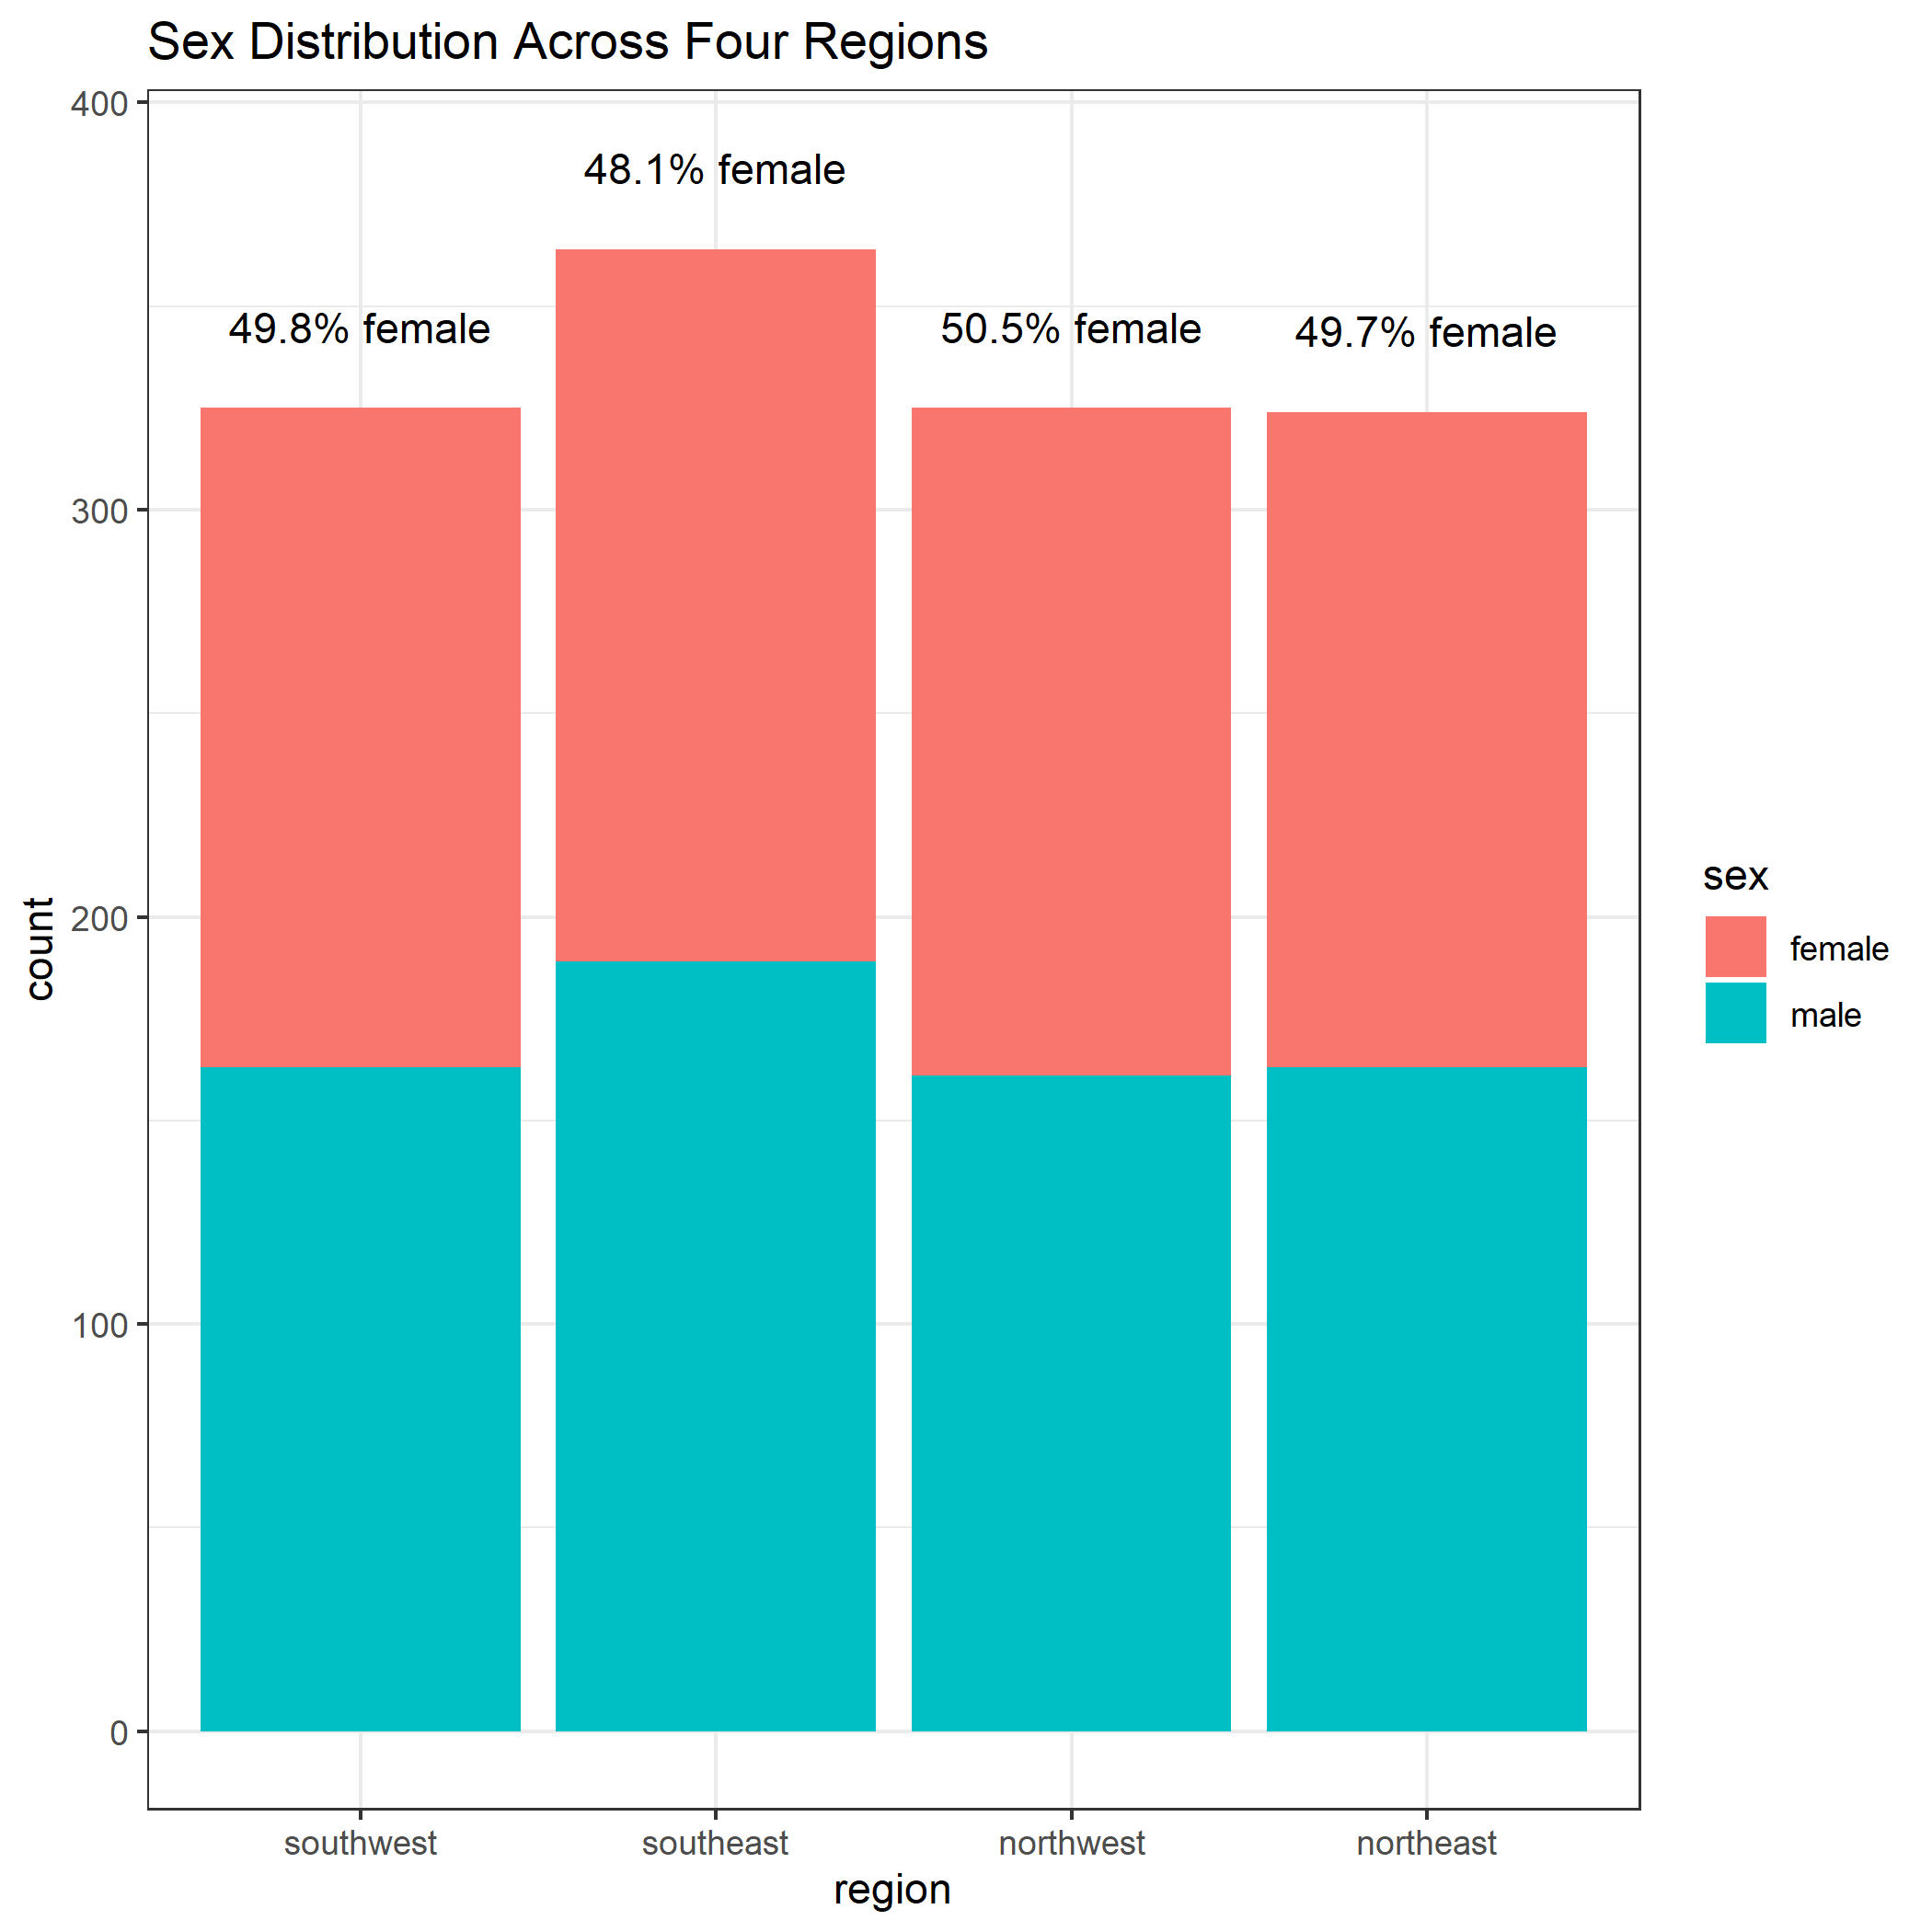
\includegraphics{../images/region_barchart.png}
\caption{Region bar chart}
\end{figure}

\hypertarget{methods}{%
\subsection{Methods}\label{methods}}

\hypertarget{results}{%
\subsection{Results}\label{results}}

\hypertarget{discussion}{%
\subsection{Discussion}\label{discussion}}

\hypertarget{references}{%
\subsection{References}\label{references}}

\begin{enumerate}
\def\labelenumi{\arabic{enumi}.}
\tightlist
\item
  Medical Costs Dataset -
  \url{https://gist.github.com/meperezcuello/82a9f1c1c473d6585e750ad2e3c05a41}
\item
  BMI -
  \url{https://www.nhlbi.nih.gov/health/educational/lose_wt/BMI/bmi-m.htm}
\end{enumerate}

\end{document}
